\section{Long-Context Architectures}

\begin{frame}{}
    \LARGE Next-Generation Architectures: \textbf{Long Context}

    \vspace{1em}
    \normalsize We can now afford a million tokens. Can the model actually use them?
\end{frame}

\begin{frame}{Three Things Break When Context Grows}
    \begin{enumerate}\itemsep0.8em
        \item \textbf{Positions.} The model meets position indices it never saw in training. With RoPE, that means rotation angles outside the trained range.
        \item \textbf{Attention itself.} Trained heads rely on habits, such as dumping spare attention on the first token. Change the window and those habits fail.
        \item \textbf{Finding things.} Even when nothing breaks, retrieving the right fact among a million tokens is hard. And we need honest ways to measure it.
    \end{enumerate}
    \vspace{0.8em}
    \takeaway{This section follows that order: \textbf{extend the positions}, \textbf{engineer the sinks}, then \textbf{train and evaluate} at 1M tokens.}
\end{frame}

\subsection{Positions and Attention Sinks}

\begin{frame}{Why RoPE Fails Beyond Its Training Length}
    \begin{columns}[T,onlytextwidth]
        \column{0.56\textwidth}
        \begin{itemize}\itemsep0.45em
            \item RoPE rotates each pair of dimensions at its own frequency. Dimension $d$ has wavelength
            \[ \lambda_d = 2\pi\, b^{\,2d/|D|} \]
            \item \textbf{Fast} dimensions complete many rotations inside the training length $L$. They have seen every angle.
            \item \textbf{Slow} dimensions never finish one rotation. Past $L$ they produce angles the model has \alert{never seen}.
            \item \textbf{Position Interpolation:} squeeze new positions into the old range, $m \mapsto mL/L'$. It works after a short fine-tune, but it also squeezes the fast dimensions, which blurs \emph{local} order.
        \end{itemize}
        \column{0.42\textwidth}
        \centering
        \begin{adjustbox}{max width=\linewidth}\begin{tikzpicture}
            \begin{axis}[width=6.3cm, height=5.0cm,
                xlabel={\scriptsize rotations completed within $L$}, ylabel={\scriptsize frequency multiplier},
                xmode=log, xmin=0.05, xmax=1000, ymin=0, ymax=1.15,
                xtick={0.1,1,32,1000}, xticklabels={0.1,1,32,1000},
                ytick={0.125,1}, yticklabels={$1/s$,1},
                tick label style={font=\scriptsize}, legend style={font=\scriptsize, at={(0.03,0.6)}, anchor=west, draw=none, fill=none},
                axis lines=left]
                \addplot[KAred, thick, dashed] coordinates {(0.05,0.125) (1000,0.125)};
                \addlegendentry{PI: all equal}
                \addplot[KAUSTblue, very thick] coordinates {(0.05,0.125) (1,0.125) (2,0.153) (4,0.210) (8,0.323) (16,0.548) (32,1) (1000,1)};
                \addlegendentry{YaRN: by band}
            \end{axis}
        \end{tikzpicture}\end{adjustbox}

        {\scriptsize Schematic from the YaRN ramp with $\alpha=1$, $\beta=32$, $s=8$.}
    \end{columns}
    \src{Chen et al., ``Extending Context Window of Large Language Models via Positional Interpolation,'' \href{https://arxiv.org/abs/2306.15595}{arXiv:2306.15595}. Peng et al., ``YaRN,'' \href{https://arxiv.org/abs/2309.00071}{arXiv:2309.00071}.}
\end{frame}

\begin{frame}{YaRN: Treat Each Frequency Band Differently}
    \begin{itemize}\itemsep0.29em
        \item Let $r(d)=L/\lambda_d$ be the rotations a dimension completes in training. YaRN blends per dimension:
        \[
            \theta_d' = \big(1-\gamma(r)\big)\frac{\theta_d}{s} + \gamma(r)\,\theta_d,
            \qquad
            \gamma(r)=\begin{cases}0 & r<\alpha\\ 1 & r>\beta\\ \frac{r-\alpha}{\beta-\alpha} & \text{otherwise}\end{cases}
        \]
        \item \textbf{Fast dimensions} are left alone. \textbf{Slow dimensions} are fully interpolated. The rest are blended.
        \item Longer contexts also flatten attention, so YaRN adds a temperature, $\sqrt{1/t}=0.1\ln s+1$.
        \item \textbf{Cost:} about 400 fine-tuning steps, against 1,000 for Position Interpolation.
    \end{itemize}
    \vspace{0.13em}
    \takeaway{\textbf{Still in use in 2026.} gpt-oss, Qwen3-Next and DeepSeek-V4 all ship with YaRN scaling in their configurations.}
    \src{Peng et al., ``YaRN: Efficient Context Window Extension of Large Language Models,'' \href{https://arxiv.org/abs/2309.00071}{arXiv:2309.00071}. Model cards and configurations of gpt-oss, Qwen3-Next and DeepSeek-V4.}
\end{frame}

\begin{frame}{After YaRN: Search It, Train It, or Remove It}
    \begin{itemize}\itemsep0.6em
        \item \textbf{Search it.} \emph{LongRoPE} finds a separate scale for every dimension by evolutionary search, and reaches 2M tokens. \emph{LongRoPE2} adds one insight: slow dimensions are under-trained, so the cut-off sits earlier than theory says. On Llama-3-8B at 128K it scores 82.0 on RULER with \textbf{10B} tokens of training. Meta used 800B.
        \item \textbf{Train it.} Frontier labs now build extension into pre-training. They raise the RoPE base (Llama 3 uses 500,000) and lengthen sequences in stages.
        \item \textbf{Remove it.} A growing group uses \alert{no positional encoding} in the global-attention layers, and leaves order to local or recurrent layers:
        \begin{itemize}\itemsep0.2em
            \item Llama 4 interleaves NoPE layers with RoPE layers
            \item Nemotron 3 and Kimi Linear: the recurrent layers already encode order
            \item DeepSeek-V4 and Qwen3-Next apply RoPE to only a fraction of the dimensions
        \end{itemize}
    \end{itemize}
    \src{Ding et al., ``LongRoPE,'' \href{https://arxiv.org/abs/2402.13753}{arXiv:2402.13753}. Shang et al., ``LongRoPE2,'' \href{https://arxiv.org/abs/2502.20082}{arXiv:2502.20082}, Table 2. Meta, \href{https://arxiv.org/abs/2407.21783}{arXiv:2407.21783} and Llama 4 blog (2025). NVIDIA, \href{https://arxiv.org/abs/2512.20856}{arXiv:2512.20856}.}
\end{frame}

\begin{frame}{Engineering the Attention Sink}
    \begin{columns}[T,onlytextwidth]
        \column{0.5\textwidth}
        \begin{itemize}\itemsep0.2em
            \item Sinks get \textbf{stronger} with longer training context and larger models, so recent designs build in a ``do nothing'' option.
            \item \textbf{Fix A: give it a real null slot.} Add a learned term to the denominator (gpt-oss, DeepSeek-V4):
            \[
                a_{ij}=\frac{e^{z_{ij}}}{\sum_k e^{z_{ik}}+e^{z'}}
            \]
            with $z_{ij}$ the attention logits and $z'$ a learned logit per head.
            \item \textbf{Fix B: let the head switch off.} Gate the attention output, $Y'=Y\odot\sigma(XW_\theta)$ (Qwen).
        \end{itemize}
        \column{0.48\textwidth}
        \centering
        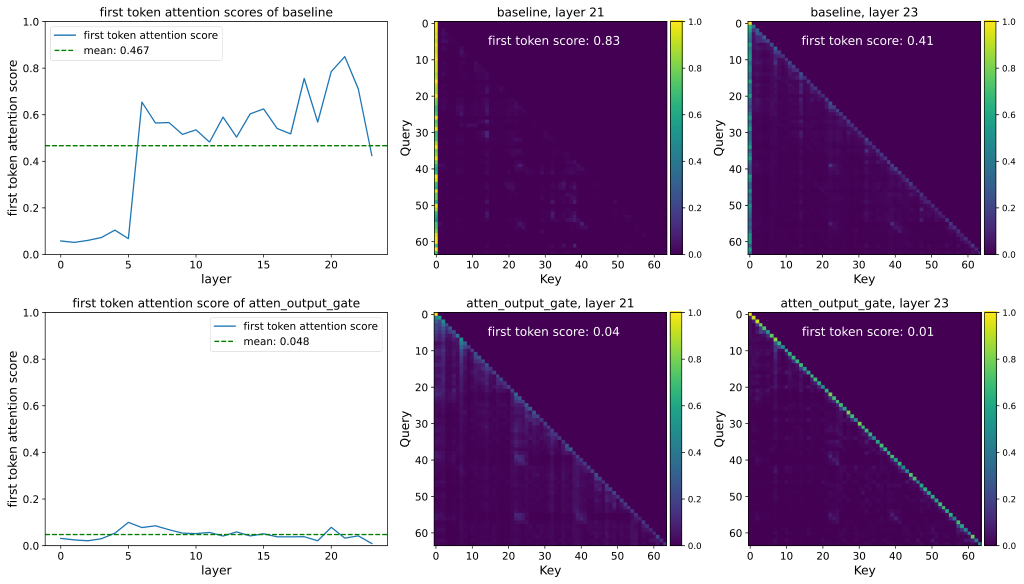
\includegraphics[width=\linewidth,height=0.44\textheight,keepaspectratio]{images/next-gen-architectures/gated_attention_fig_attn_scores.png}

        {\scriptsize With output gating, mean first-token attention falls from 0.467 to 0.048.}
    \end{columns}
    \src{Barbero et al., ``Why do LLMs attend to the first token?'' \href{https://arxiv.org/abs/2504.02732}{arXiv:2504.02732}. DeepSeek-V4, \href{https://arxiv.org/abs/2606.19348}{arXiv:2606.19348}, Eq. 27. Figure: Qiu et al., ``Gated Attention for Large Language Models,'' \href{https://arxiv.org/abs/2505.06708}{arXiv:2505.06708}.}
\end{frame}

\subsection{Training and Evaluating at 1M Tokens}

\begin{frame}{How Models Are Actually Trained to 1M Tokens}
    \begin{center}
    \small
    \renewcommand{\arraystretch}{1.25}
    \begin{adjustbox}{max width=\linewidth}\begin{tabular}{lll}
        \toprule
        \textbf{Model} & \textbf{Length schedule} & \textbf{Tokens spent on long stages} \\
        \midrule
        Llama 3 (2024) & 6 stages, 8K to 128K & about 800B \\
        MiniMax-01 (2025) & 128K, then 512K, then 1M & 300B + 32B + 26B \\
        Nemotron 3 Super (2026) & 8K, then straight to 1M & 34B + 17B \\
        DeepSeek-V4 (2026) & 4K, 16K, 64K, then 1M & not reported per stage \\
        \bottomrule
    \end{tabular}\end{adjustbox}
    \end{center}
    \begin{itemize}\itemsep0.4em
        \item \textbf{The last stage is cheap.} A few tens of billions of tokens at 1M, after trillions at short length.
        \item \textbf{Gate each stage.} Llama 3 moved on only when short-context quality had recovered \emph{and} needle retrieval was perfect at the new length.
        \item \textbf{Needle tests saturate early.} MiniMax found them solved long before real long-context ability appeared, and tracked harder tasks instead.
    \end{itemize}
    \src{Meta, \href{https://arxiv.org/abs/2407.21783}{arXiv:2407.21783}. MiniMax, \href{https://arxiv.org/abs/2501.08313}{arXiv:2501.08313}, Table 6. NVIDIA, ``Nemotron 3 Super,'' \href{https://arxiv.org/abs/2604.12374}{arXiv:2604.12374}. DeepSeek-AI, \href{https://arxiv.org/abs/2606.19348}{arXiv:2606.19348}.}
\end{frame}

\begin{frame}{The 2026 Picture: What Happens Between 128K and 1M}
    \begin{columns}[T,onlytextwidth]
        \column{0.5\textwidth}
        \centering
        \small
        \begin{adjustbox}{max width=\linewidth}\begin{tabular}{lccc}
            \toprule
            \textbf{Model} & \textbf{to 128K} & \textbf{to 1M} & \textbf{Decay} \\
            \midrule
            Claude Opus 4.6 & 77.1 & 70.6 & 8.5\% \\
            Gemini 3.1 Pro & 77.8 & 68.5 & 12.0\% \\
            GPT-5.5 & 74.6 & 67.8 & 9.2\% \\
            DeepSeek-V4-Pro & 71.6 & 59.1 & 17.4\% \\
            Qwen3.5-397B & 71.0 & 54.4 & 23.3\% \\
            GLM-5 & 64.3 & 44.3 & 31.1\% \\
            \bottomrule
        \end{tabular}\end{adjustbox}

        \vspace{0.3em}
        {\scriptsize ATLAS score, averaged over lengths from 8K up to the stated limit.}
        \column{0.48\textwidth}
        \begin{itemize}\itemsep0.45em
            \item An \textbf{independent} harness over 26 models: the average score drops \alert{24.3\%} when the range extends from 128K to 1M.
            \item Retrieval and question answering lose the most at 1M.
            \item Closed frontier models decay by 8 to 14\%. Open models by 17 to 60\%.
            \item \textbf{Beware vendor tables.} Labs report the same benchmark in different formats, and their numbers for each other's models disagree.
        \end{itemize}
    \end{columns}
    \vspace{0.4em}
    \takeaway{A 1M-token window is real. Uniform quality across that window is not there yet.}
    \src{Huang et al., ``ATLAS,'' \href{https://arxiv.org/abs/2605.28079}{arXiv:2605.28079}, Tables 10 and 11 (May 2026).}
\end{frame}

\begin{frame}{Long Context: What to Remember}
    \begin{itemize}\itemsep0.6em
        \item \textbf{Positions:} scale RoPE by frequency band (YaRN), or drop positional encoding from global layers altogether.
        \item \textbf{Sinks:} softmax needs a ``do nothing'' option. Modern models provide one on purpose.
        \item \textbf{Training:} stage the length, gate each stage, and spend little at the longest length.
        \item \textbf{Evaluation:} trust independent, reasoning-heavy benchmarks over needle tests and vendor tables.
    \end{itemize}
    \vspace{0.4em}
    \takeaway{\textbf{Next.} Every design so far changes what a parameter or a token costs. How should a fixed budget be divided between model size, data and inference?}
\end{frame}
